\documentclass[a4paper,12pt]{article}


\input{lab_Preamble.tex}
\mathtoolsset{showonlyrefs}

\begin{document}

\begin{titlepage}
	\begin{center}
		
		\textsc{\LARGE Московский\\[-0.2cm]Физико-Технический Институт\\[0.1cm]\large (национальный исследовательский университет)}\\[1.5cm] 
		
	\includegraphics[width=0.3\textwidth]{hv_s_no_bg.png}~\\[1cm]

	\textsc{\Large Оптика. \\ Лабораторный практикум. }\\[0.2cm]

	% Title
	\HRule \\[0.4cm]
	{ \LARGE \bfseries Лабораторная работа № 4.2.1 \\ Кольца Ньютона. \\[0.4cm] }

	\HRule \\[1.5cm]
		
		% Author and supervisor
		\noindent
		\begin{minipage}{0.4\textwidth}
			\begin{flushleft} \large
			\end{flushleft}
		\end{minipage}%
		\begin{minipage}{0.4\textwidth}
			\begin{flushright} \large
			\end{flushright}
		\end{minipage}
		
		
		\large{\begin{flushright}
				\vfill
				\textbf{Выполнили}:\\
				\textbf{Рябых Владислав,\\}
				\textbf{Исыпов Илья\\}
				\textbf{группа Б05-905}
		\end{flushright}}
		
		
		{\large \today}\\
		
		
	\end{center}
\end{titlepage}

\subsubsection*{Цель работы:} познакомиться с явлением интерференции в тонких плёнках (полосы равной толщины) на примере колец Ньютона и с методикой интерференционных измерений кривизны стеклянной поверхности.талл; наблюдать изменение характера поляризации света при наложении на кристалл электрического поля.

\subsubsection*{Оборудование:} измерительный микроскоп с опак-иллюминатором, плоско-выпуклая линза; пластинка из чёрного стекла, ртутная лампа типа ДРШ, щель, линзы, призма прямого зрения, объектная шкала.

\section*{Теория}

\begin{wrapfigure}{l}{0.35\linewidth} 
	\includegraphics[width=\linewidth]{ring}
	\caption{Экспериментальная установка}
	\label{ring}
\end{wrapfigure}

Этот классический опыт используется для определения радиуса кривизны сферических поверхностей линз. В этом опыте наблюдается интерференция волн, отражённых от границ тонкой воздушной прослойки, образованной сферической поверхностью линзы и плоской стеклянной пластиной. При нормальном падении света (рис. \ref{ring}) интерференционные полосы локализованы на сферической поверхности и являются полосами равной толщины.

Геометрическая разность хода между интерферирующими лучами равна удвоенной толщине воздушного зазора $ 2d $ в данном месте. Для точки на сферической поверхности, находящейся на расстоянии $ r $ от оси системы, имеем $ r^2 = R^2 - (R - d)^2 = 2Rd - d^2 $, где $ R $ --- радиус кривизны сферической поверхности (рис. \ref{ring}).

При $ R \gg d $ получим$  d = r^2/2R $. С учётом изменения фазы на $ \pi $ при отражении волны от оптически более плотной среды (на границе воздух-стекло) получим \textbf{оптическую разность хода интерферирующих лучей}:

\begin{equation}\label{r_m}
\Delta = \dfrac{\lambda}{2} + 2d = \dfrac{r^2}{2R} + \dfrac{\lambda}{2}
\end{equation}

Из условия интерференционного минимума $ \Delta = \dfrac{(2m +1)\lambda}{2}, \; m =0, 1, 2.. $ получим радиусы темных колец $ r_m $, а из аналогичного условия максимума $ \Delta = m \lambda $ радиусы светлых $ r_m' $ :

\begin{equation}\label{r_m'}
r_m = \sqrt{m \lambda R}, \qquad 	r_m' = \sqrt{\dfrac{(2m-1)m \lambda R}{2}}
\end{equation}

\section*{Экспериментальная установка}

Схема экспериментальной установки приведена на рис. \ref{lab}. Опыт выполняется с помощью измерительного микроскопа.
На столик микроскопа помещается держатель с полированной пластинкой из
чёрного стекла. На пластинке лежит исследуемая линза.

\begin{wrapfigure}{r}{0.5\linewidth} 
	\includegraphics[width=\linewidth]{lab}
	\caption{Экспериментальная установка}
	\label{lab}
\end{wrapfigure}

Источником света служит ртутная лампа, находящаяся в защитном кожухе. Для получения монохроматического света применяется призменный монохроматор, состоящий из конденсора $ К $, коллиматора (щель $ S $ и объектив $ О $) и призмы прямого зрения $ П $. Эти устройства с помощью рейтеров располагаются на оптической скамье. Свет от монохроматора попадает на расположенный между объективом и окуляром микроскопа опак-иллюминатор (ОИ)  специальное устройство, служащее для освещения объекта при работе в отражённом свете. Внутри опак-иллюминатора находится полупрозрачная стеклянная пластинка P, наклоненная под углом $ 45^\circ $ к оптической оси микроскопа. Свет частично отражается от этой пластинки, проходит через объектив микроскопа и попадает на исследуемый объект. Пластинка может поворачиваться вокруг горизонтальной оси $ X $, опак-иллюминатор вокруг вертикальной оси.

Столик микроскопа может перемещаться в двух взаимно перпендикулярных направлениях с помощью винтов препаратоводителя. Отсчётный крест окулярной шкалы перемещается перпендикулярно оптической оси с помощью микрометрического винта $ М $.

Оптическая схема монохроматора позволяет получить в плоскости входного окна опак-иллюминатора достаточно хорошо разделённые линии спектра ртутной лампы. Изображение щели $ S $ фокусируется на поверхность линзы объективом микроскопа, т.е. точка источника и точка наблюдения спектра совпадают. Интерференционная картина не зависит от показателя преломления линзы и определяется величиной зазора между линзой и пластинкой (кольца равной толщины).

Сначала микроскоп настраивается на кольца Ньютона в белом свете (свете ртутной лампы), затем при помощи монохроматора выделить из спектра яркую зелёную линию и провести измерения диаметров колец в монохроматическом свете. 


\section*{Ход работы}

После настройки микроскопа проведем измерения диаметров колец Ньютона. Измерения будем проводить в безразмерных единицах окулярной шкалы, переведённых затем в реальную величину с помощью калиброванной объектной шкалы. 


Оценим систематическую погрешность измерения величин на окуляре как $ \sigma = 0.02 $ (из-за цены деления).

C помощью призмы разобьем свет ртутной лампы на зеленый ($ \lambda_\text{з} = 546 $ нм) и желтый ($ \lambda_\text{ж} = 578  $ нм).

Будем последовательно измерять координаты колец. Вычтем из них координату центра, возьмём по модулю~---~ получим радиусы колец, занесём их в таблицу \ref{circles}. 

\begin{center}
	\begin{tabular}{|c|c|c|c|c|}
			\hline
			& \multicolumn{2}{|c|}{Светлые кольца} & \multicolumn{2}{|c|}{Тёмные кольца} \\
			\hline
			$m$ & $ r_m' $ & $ (r_m')^2 $ & $ r_m $ & $ (r_m)^2 $ \\
			\hline
			
			1 & 0.2 & 0.04 & 0.58 & 0.34  \\
			2 & 0.73 & 0.53 & 1.03 & 1.06  \\
			3 & 1.16 & 1.35 & 1.35 & 1.82  \\
			4 & 1.49 & 2.22 & 1.67 & 2.79 \\
			5 & 1.76 & 3.1 & 1.89  & 3.57  \\
			6 & 1.98 & 3.92 &  &  \\
			
			\hline
		\end{tabular}
	\captionof{table}{Измерение радиусов колец Ньютона}\label{circles}
\end{center}

Построим график зависимости радиусов колец от их номера, см. рис. \ref{graf}.

\begin{center}
	\begin{figure}[hbt!]
		\centering
		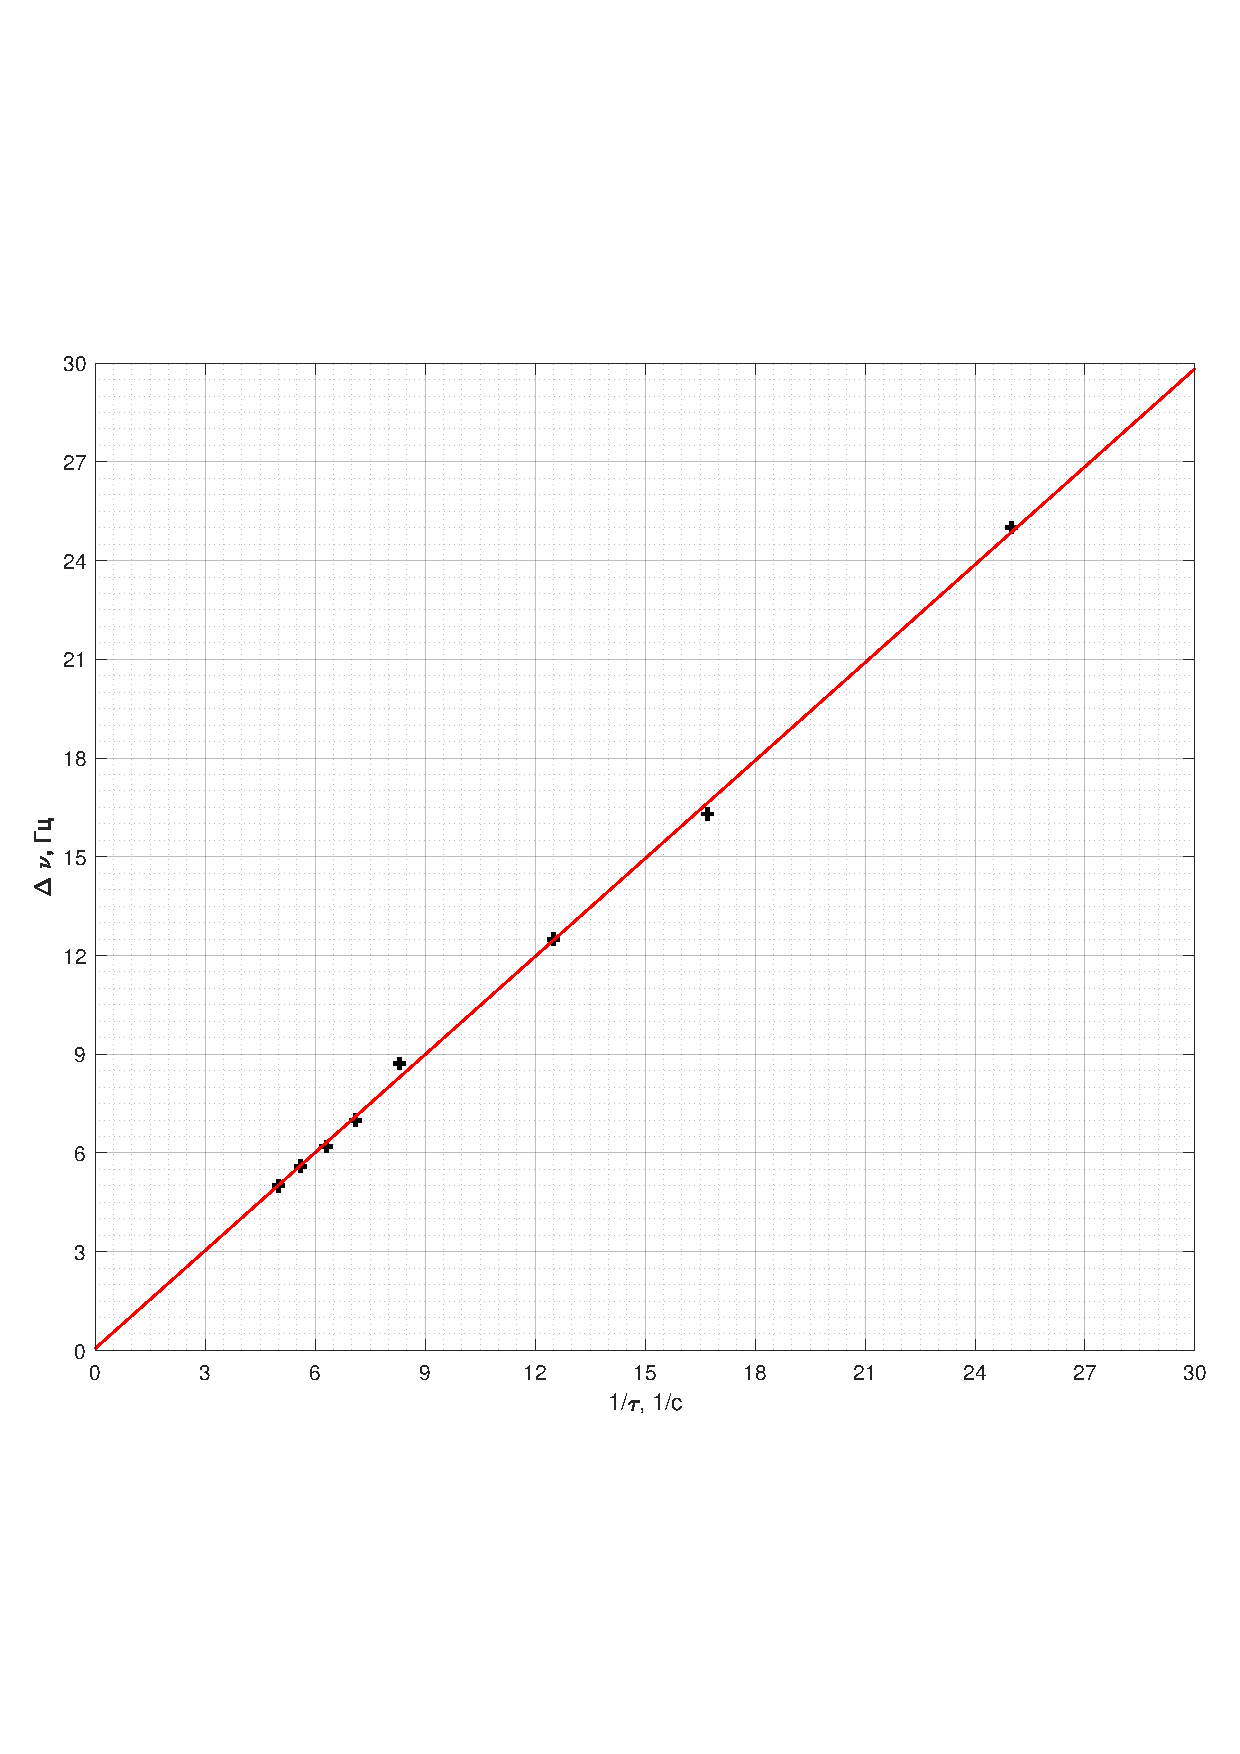
\includegraphics[width=\linewidth]{gr1.pdf}
		\caption{График зависимости $r_m^2$ и $(r_m')^2$ от номера $m$}
		\label{graf}
	\end{figure}
\end{center}
 
По МНК получаем: 

\begin{center}
	\begin{tabular}{c|c}
%		\hline
		тёмные кольца & $0.82x-0.54 $ \\
		\hline
		светлые кольца & $0.80x-0.94 $ \\
%		\hline
	\end{tabular}
\end{center}
	

Теперь определим калибровку окулярной шкалы. Она равна $ k = 0.11 $ мм.

При биениях мы наблюдали $ \Delta m =  12 $ полос между центрами четких систем. Вычислим отсюда разность длин волн желтого и зеленого света ртутной лампы $ \Delta \lambda = \lambda_\text{ж} - \lambda_\text{з} $:

\begin{equation}
(\Delta m + 1)\lambda_\text{з} = \Delta m \lambda_\text{ж} \Ra \Delta \lambda = \dfrac{\lambda_\text{з}}{\Delta m} \approx 45 \; \text{нм}
\end{equation}

Определим радиус кривизны линзы. Так как $ \dfrac{r^2_m}{m} = k^2 \cdot a_\text{т}$, отсюда

\begin{equation}
R = \dfrac{r^2_m}{m \lambda} = (1.81 \pm 0.03) \; \text{см}
\end{equation}


\section*{Вывод}

Экспериментально мы получили, что разница длин волн жёлтого и зелёного цвета ртутной лампы составила $  \Delta \lambda = 45$ нм, что относительно близко к табличным данным (33 нм).

Также мы  получили кольца Ньютона как результат интерференции света, построили графики зависимости квадрата радиуса кольца Ньютона от его номера. По данным графика мы рассчитали радиус кривизны линзы $ R = (1.81 \pm 0.03) \; \text{см} $.

\end{document}